%%%%%%%%%%%%%%%%%%%%%%%%%%%%%%%%%%%%%%%%%
% Beamer Presentation
% LaTeX Template
% Version 1.0 (10/11/12)
%
% This template has been downloaded from:
% http://www.LaTeXTemplates.com
%
% License:
% CC BY-NC-SA 3.0 (http://creativecommons.org/licenses/by-nc-sa/3.0/)
%
%%%%%%%%%%%%%%%%%%%%%%%%%%%%%%%%%%%%%%%%%

%----------------------------------------------------------------------------------------
%	PACKAGES AND THEMES
%----------------------------------------------------------------------------------------

\documentclass{beamer}

\mode<presentation> {

% The Beamer class comes with a number of default slide themes
% which change the colors and layouts of slides. Below this is a list
% of all the themes, uncomment each in turn to see what they look like.

\usetheme{default}
%\usetheme{AnnArbor}
%\usetheme{Antibes}
%\usetheme{Bergen}
%\usetheme{Berkeley}
%\usetheme{Berlin}
%\usetheme{Boadilla}
%\usetheme{CambridgeUS}
%\usetheme{Copenhagen}
%\usetheme{Darmstadt}
%\usetheme{Dresden}
%\usetheme{Frankfurt}
%\usetheme{Goettingen}
%\usetheme{Hannover}
%\usetheme{Ilmenau}
%\usetheme{JuanLesPins}
%\usetheme{Luebeck}
%\usetheme{Madrid}
%\usetheme{Malmoe}
%\usetheme{Marburg}
%\usetheme{Montpellier}
%\usetheme{PaloAlto}
%\usetheme{Pittsburgh}
%\usetheme{Rochester}
%\usetheme{Singapore}
%\usetheme{Szeged}
%\usetheme{Warsaw}

% As well as themes, the Beamer class has a number of color themes
% for any slide theme. Uncomment each of these in turn to see how it
% changes the colors of your current slide theme.

%\usecolortheme{albatross}
%\usecolortheme{beaver}
%\usecolortheme{beetle}
%\usecolortheme{crane}
%\usecolortheme{dolphin}
%\usecolortheme{dove}
%\usecolortheme{fly}
%\usecolortheme{lily}
%\usecolortheme{orchid}
%\usecolortheme{rose}
%\usecolortheme{seagull}
%\usecolortheme{seahorse}
%\usecolortheme{whale}
%\usecolortheme{wolverine}

%\setbeamertemplate{footline} % To remove the footer line in all slides uncomment this line
%\setbeamertemplate{footline}[page number] % To replace the footer line in all slides with a simple slide count uncomment this line

%\setbeamertemplate{navigation symbols}{} % To remove the navigation symbols from the bottom of all slides uncomment this line
}

\usepackage{graphicx} % Allows including images
\usepackage{booktabs} % Allows the use of \toprule, \midrule and \bottomrule in tables
\usepackage{url}
\usepackage[T1]{fontenc}
\usepackage[utf8]{inputenc}
\usepackage{listings}
\usepackage{adjustbox}
\lstset{language=C++,
  basicstyle=\footnotesize\ttfamily,
  keywordstyle=\footnotesize\color{blue}\ttfamily,
}
%----------------------------------------------------------------------------------------
%	TITLE PAGE
%----------------------------------------------------------------------------------------

\title[Lab 7]{Lab 7} % The short title appears at the bottom of every slide, the full title is only on the title page

\author{Kasper Høj Lorenzen} % Your name
\institute[SDU Robotics] % Your institution as it will appear on the bottom of every slide, may be shorthand to save space
{
University of Southern Denmark \\ % Your institution for the title page
\medskip
\textit{kalor@mmmi.sdu.dk} % Your email address
}
\date{October 27, 2022} % Date, can be changed to a custom date

\begin{document}

\begin{frame}
\titlepage % Print the title page as the first slide
\end{frame}

\begin{frame}
\frametitle{Overview} % Table of contents slide, comment this block out to remove it
\tableofcontents % Throughout your presentation, if you choose to use \section{} and \subsection{} commands, these will automatically be printed on this slide as an overview of your presentation
\end{frame}

%----------------------------------------------------------------------------------------
%	PRESENTATION SLIDES
%----------------------------------------------------------------------------------------

% ------------------------------------------------
\section{General Comments}
% ------------------------------------------------

\begin{frame}
  \frametitle{General Comments}
  \begin{columns}
    \begin{column}{0.4\textwidth}
      \begin{center}
        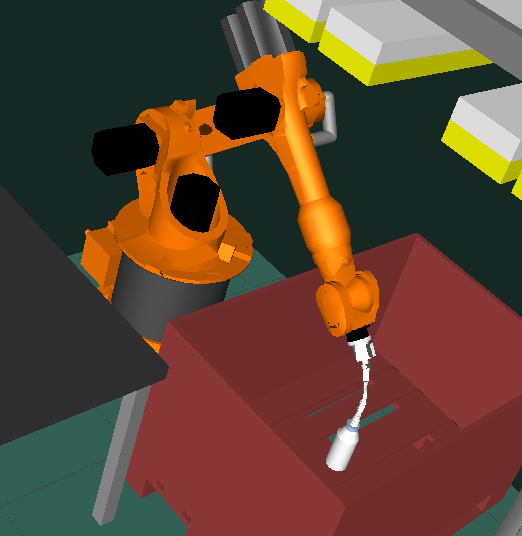
\includegraphics[width=\textwidth]{./pick}
      \end{center}
    \end{column}
    \begin{column}{0.6\textwidth}
      \begin{itemize}
      \item Why does the robot make a big circle in all paths?
      \end{itemize}
      \begin{center}
        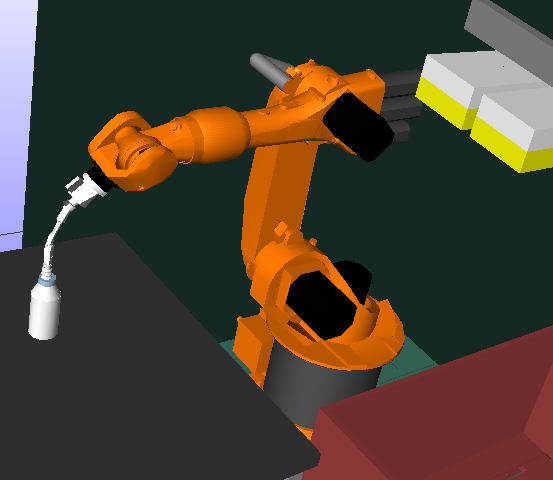
\includegraphics[width=0.6666\textwidth]{./place}
      \end{center}
    \end{column}
  \end{columns}
\end{frame}


\begin{frame}
  \frametitle{General Comments}
  \begin{columns}
    \begin{column}{0.4\textwidth}
      \begin{center}
        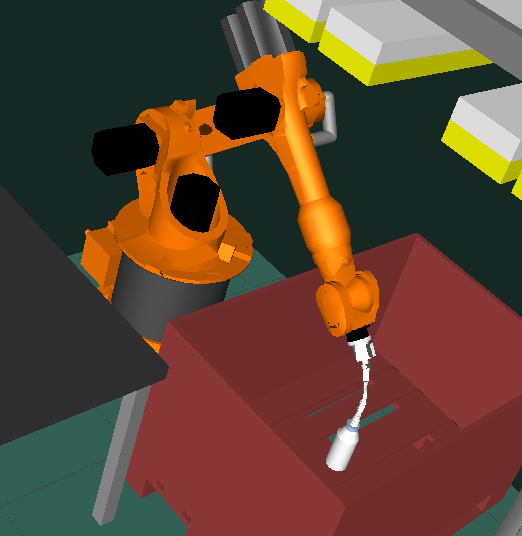
\includegraphics[width=\textwidth]{./pick}
      \end{center}
    \end{column}
    \begin{column}{0.6\textwidth}
      \begin{itemize}
      \item Why does the robot make a big circle in all paths?
        \begin{itemize}
        \item The base joint needs to turn $180^{\circ}$ to reach the place position.
        \end{itemize}
      \end{itemize}
      \begin{center}
        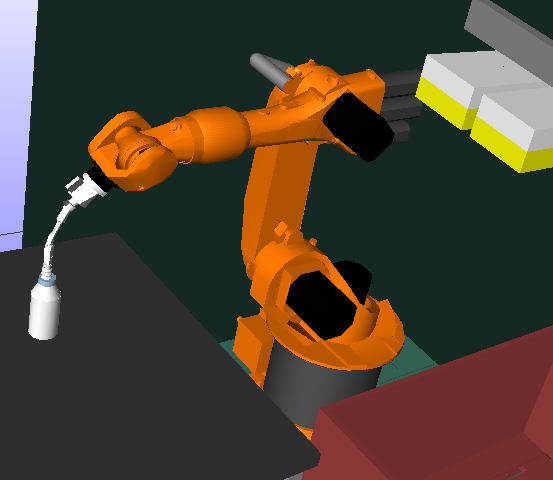
\includegraphics[width=0.6666\textwidth]{./place}
      \end{center}
    \end{column}
  \end{columns}
\end{frame}



%------------------------------------------------
%\section{C++ in RobWork}
%% ------------------------------------------------
%
%\begin{frame}
%  \frametitle{C++ in RobWork}
%  \begin{columns}
%    \begin{column}{0.4\textwidth}
%      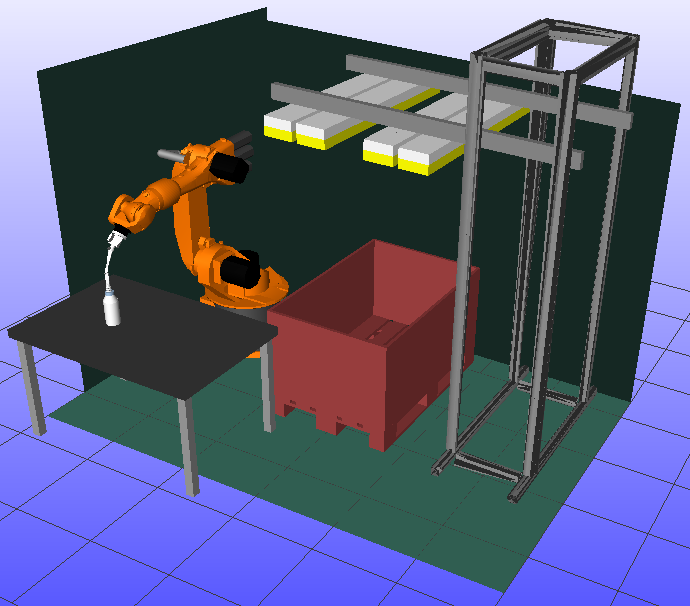
\includegraphics[width=\textwidth]{../graphics/mandEx2WC}
%    \end{column}
%    \begin{column}{0.6\textwidth}
%      \begin{itemize}
%      \item Remove const from the state and move robot to positions
%      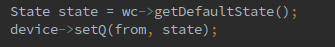
\includegraphics[width=\textwidth]{../graphics/code1}
%      \item Find and grasp the bottle before initializing planner
%      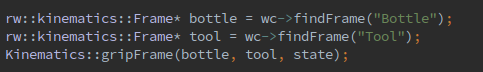
\includegraphics[width=\textwidth]{../graphics/code2}
%      \item Path length:
%        \begin{itemize}
%        \item Built-in path analyzer, or:
%          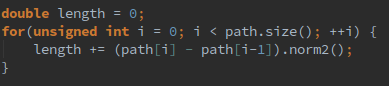
\includegraphics[width=0.75\textwidth]{../graphics/code3}
%        \end{itemize}
%      \end{itemize}
%    \end{column}
%  \end{columns}
%\end{frame}

% ------------------------------------------------
\section{$\epsilon$}
% ------------------------------------------------

\begin{frame}
  \frametitle{$\epsilon$ - Statistical Analysis}
  \begin{columns}
    \begin{column}{0.5\textwidth}
      \begin{itemize}
      \item Relevant parameters to look at:
        \begin{itemize}
        \item Path length
        \item Path size
        \item Planning time
        \end{itemize}
      \item Summary statistics
        \begin{itemize}
        \item Mean, min, max, median, quantiles
        \item Standard deviation or variance
        \end{itemize}
      \item Visualization
        \begin{itemize}
        \item Plots better than tables
          \item Box plots, scatter plots, mean line with error bars
        \end{itemize}
      \end{itemize}
    \end{column}
    \begin{column}{0.5\textwidth}
      \begin{center}
        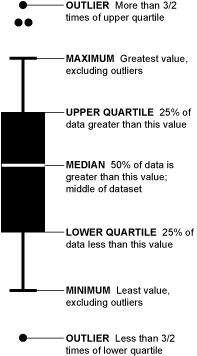
\includegraphics[scale=0.5]{./boxplot} \footnotemark
      \end{center}
    \end{column}
  \end{columns}
  \footnotetext[1]{Image borrowed from: \url{https://flowingdata.com/2008/02/15/how-to-read-and-use-a-box-and-whisker-plot/}}
\end{frame}

\begin{frame}
  \frametitle{$epsilon$ - Range}
  \begin{columns}
    \begin{column}{0.5\textwidth}
      \begin{itemize}
      \item $\epsilon$ from $0.1$ to $4.0$ in steps of $0.1$
      \end{itemize}
      \begin{center}
        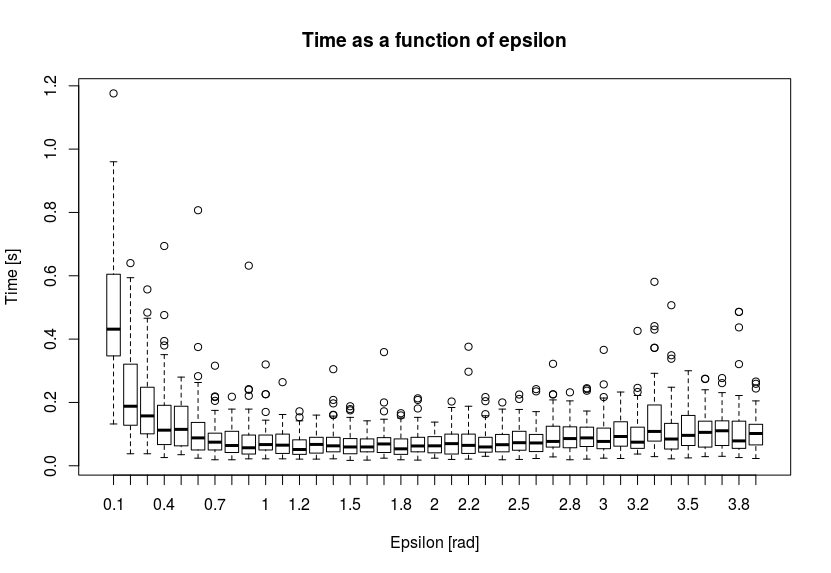
\includegraphics[width=\textwidth]{./time_v_eps_full}
      \end{center}
    \end{column}
    \begin{column}{0.5\textwidth}
      \begin{center}
        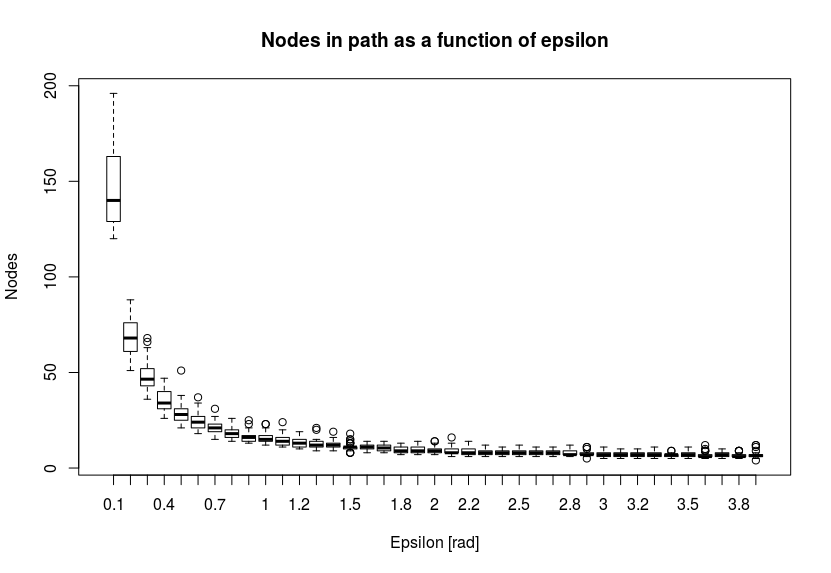
\includegraphics[width=\textwidth]{./nodes_v_eps_full}
      \end{center}
      \begin{center}
        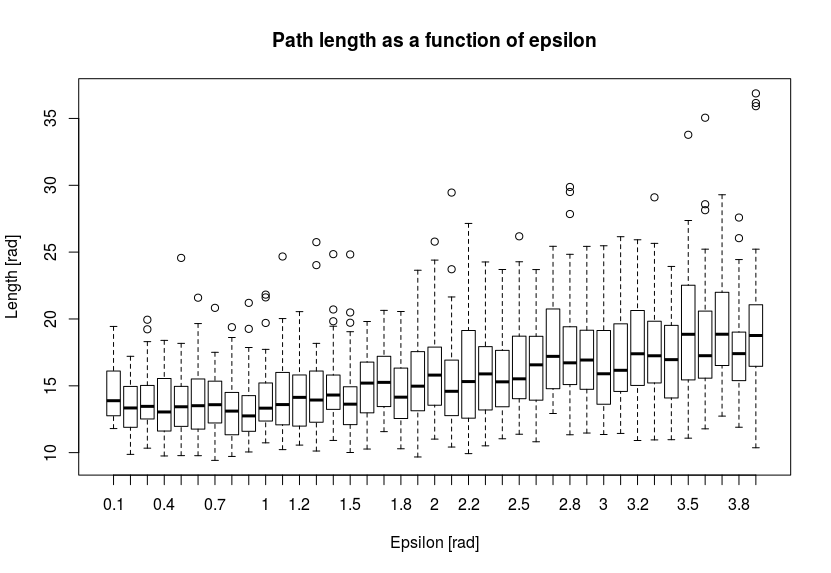
\includegraphics[width=\textwidth]{./length_v_eps_full}
      \end{center}
    \end{column}
  \end{columns}
\end{frame}


%------------------------------------------------
\section{Conclusion}
% ------------------------------------------------

\begin{frame}
  \frametitle{Conclusion}
  \begin{columns}
    \begin{column}{0.5\textwidth}
      \begin{itemize}
      \item $\epsilon$
        \begin{itemize}
        \item Trade-off between time and precision
        \item Small $\epsilon$
          \begin{itemize}
          \item Long planning time
          \item Many nodes in path
          \item Shorter path
          \end{itemize}
        \item Large $\epsilon$
          \begin{itemize}
          \item Short planning time
          \item Few nodes
          \item Longer path
          \item Might jump through obstacles 
          \end{itemize}
        \end{itemize}
      \end{itemize}
    \end{column}
    \begin{column}{0.5\textwidth}
      \begin{itemize}
      \item Choice of $\epsilon$ is workcell specific
      \item Choose $\epsilon$ based on task
      \end{itemize}
    \end{column}
  \end{columns}
\end{frame}

%------------------------------------------------
\section{Programming exercise 7}
% ------------------------------------------------

\begin{frame}
 \frametitle{Programming exercise 7 - Path Pruning}
	\begin{center}
        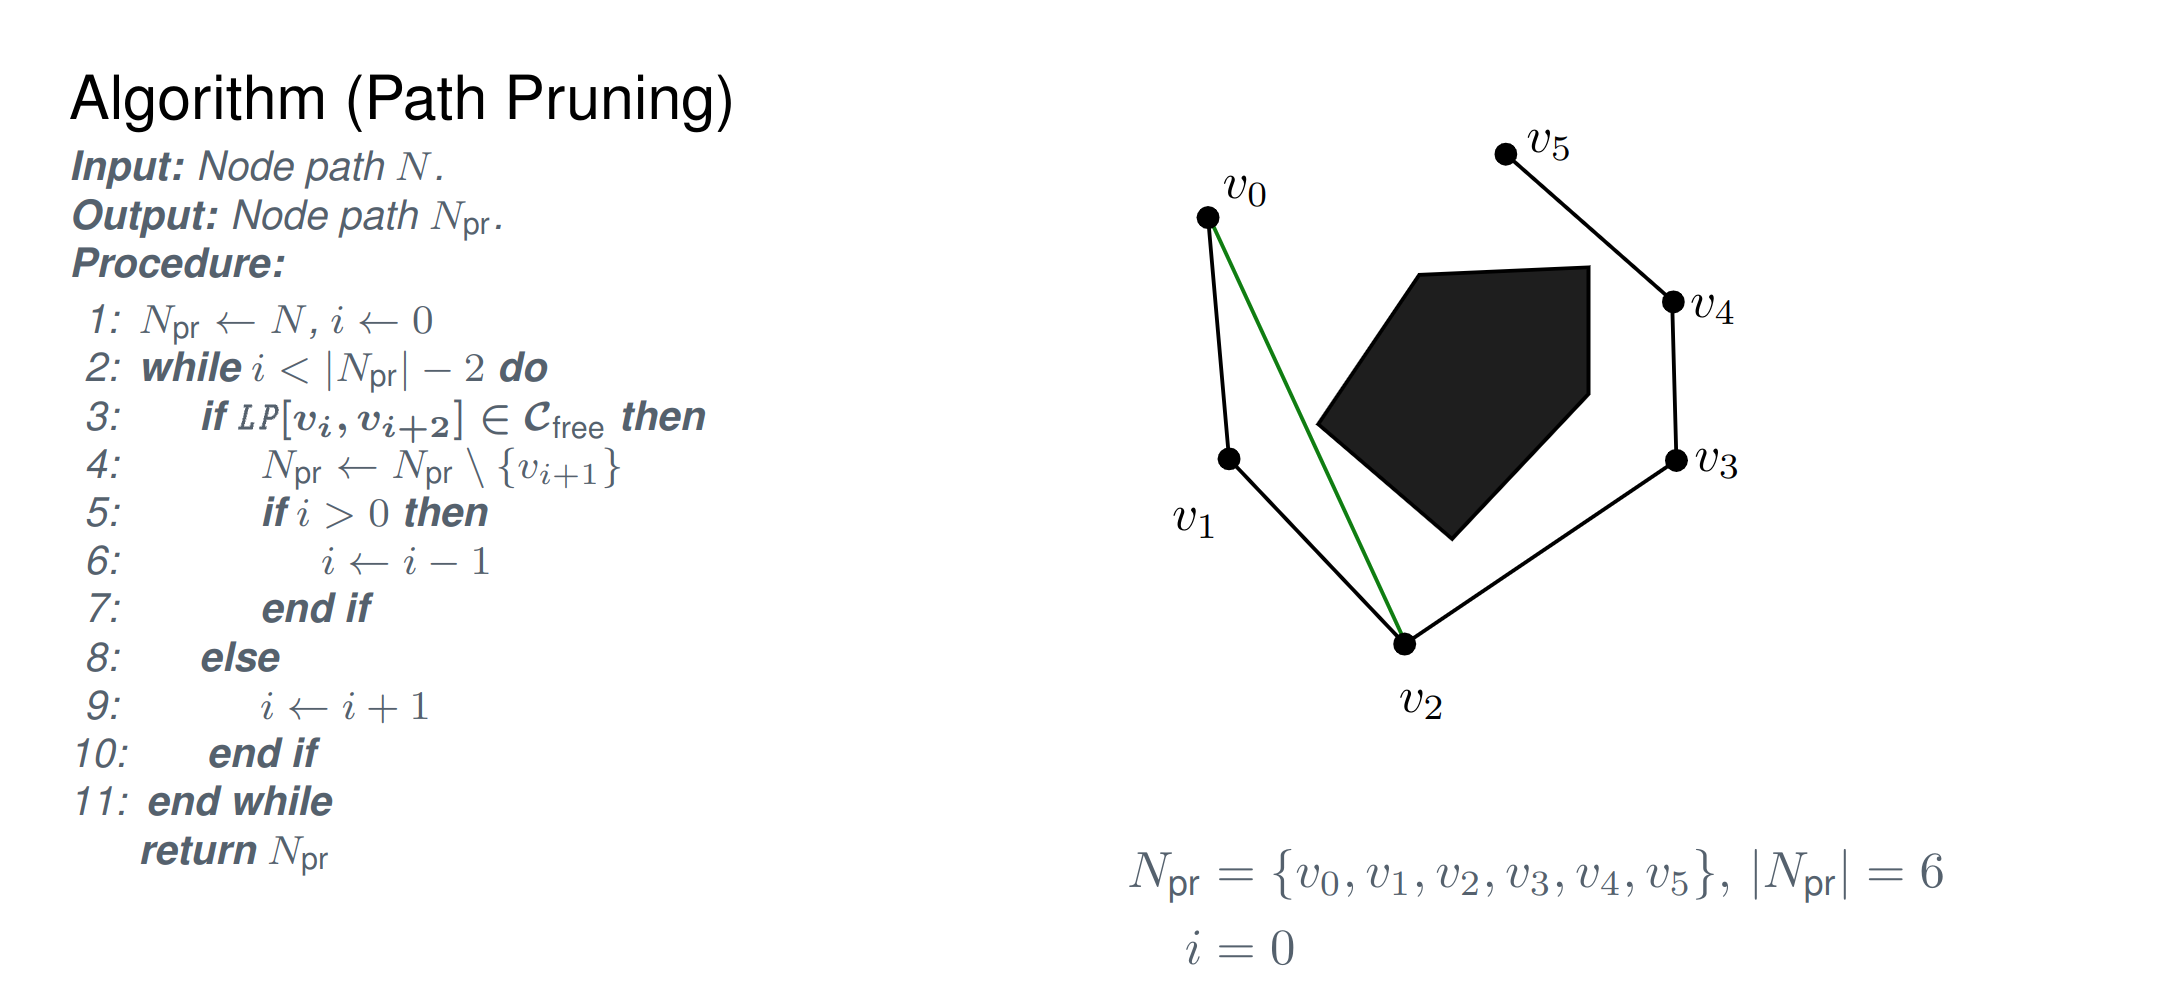
\includegraphics[width=\textwidth]{./path_pruning}
      \end{center}
\end{frame}



\begin{frame}
 \frametitle{Programming exercise 7 - Path Pruning}
  \begin{columns}
    \begin{column}{1\textwidth}
      \begin{itemize}
      \item Tips for programming exercise 7:
       \begin{itemize}
       \item Use the path that was generated in lab 6
       \item Use the workcell from lab 6 (Kr16WallWorkCell)
       \item Implement the path pruning algorithm:
       \begin{itemize}
        \item Load the workcell
        \item Loop through the Q configurations and check for collisions between the current node $Q_i$ and $Q_{i+2}$
        \item Delete node $Q_{i+1}$ if there exist a collision-free path
        \item Check the distance of the old path compared to the new one
       \end{itemize}
       \end{itemize}
      \end{itemize}
    \end{column}
  \end{columns}
\end{frame}

% \begin{frame}
%\frametitle{References}
%\footnotesize{
%\begin{thebibliography}{99} % Beamer does not support BibTeX so references must be inserted manually as below
%\bibitem[Ellekilde, Jorgensen, 2010]{robwork} L. P. Ellekilde and J. A. Jorgensen (2010)
%\newblock RobWork: A Flexible Toolbox for Robotics Research and Education
%\newblock \emph{ISR 2010 (41st International Symposium on Robotics) and ROBOTIK 2010 (6th German Conference on Robotics)}, 1 -- 7.
%\end{thebibliography}
%}
%\end{frame}

%----------------------------------------------------------------------------------------

\end{document} 
